%==================================================================================================
\chapter{Introdução}
%==================================================================================================

Problemas de interação fluido-estrutura (IFE) referem-se a situações nas quais a presença de um escoamento afeta o comportamento de uma estrutura, e vice-versa. Essa interação pode ocorrer devido ao desenvolvimento de um campo de pressões devido ao escoamento, que por sua vez solicita a estrutura, fazendo-a se deslocar, influenciando, consequentemente, o escoamento. Assim, o estudo desse tipo de problema envolve a análise multifísica, em que os diferentes meios físicos (sólido e fluido) são regidos por suas próprias equações constitutivas, e que, por sua vez, interagem entre si. Dessa forma, a análise de IFE apresenta desafios a serem superados, uma vez que envolve grande interdisciplinaridade, tanto para descrever adequadamente o comportamento dos meios físicos, quanto para se descrever como se dá essa interação.

A interação entre fluidos e estruturas é um fenômeno que ocorre em diversas situações, como em turbinas eólicas, pontes, edifícios de grande altitudes, estruturas \textit{offshore}, aeronaves, escoamento em vasos sanguíneos, entre outros. A análise desses problemas é de grande importância, uma vez que a interação entre fluidos e estruturas pode levar a falhas catastróficas, como o colapso de pontes ou edifícios, ou a perda de controle de uma aeronave.

Já em relação à classificação dos escoamentos, estes podem ser classificados, dentre outras formas, em função do número de Reynolds, o qual é um coeficiente adimensional definido como a razão entre as forças inerciais e as forças viscosas. Assim, os escoamentos podem ser classificados, a depender desse coeficiente, em 3 tipos: escoamento laminar; de transição; e turbulento. No primeiro caso, o escoamento se dá de forma similar ao escorregamento de lâminas paralelas entre si, sem que haja uma mistura macroscópica entre elas. Já no segundo caso começam a surgir algumas flutuações esporádicas no escoamento, porém ainda não se apresentam de forma tão significativa a considerá-lo turbulento. O último caso apresenta flutuações constantes em seu fluxo, resultando no surgimento de estruturas denominadas de vórtices.

Assim, em casos de escoamentos turbulentos, pode-se ocorrer o aumento do arrasto sobre a estrutura, desprendimento de vórtices, vibrações induzidas pelo escoamento, entre outros. Também pode-se ocorrer queda do coeficiente de sustentação de aerofólios, devido à formação de bolhas de desprendimento.

Com isso, pode-se partir para diferentes abordagens para obtenção de resultados para problemas de IFE. Uma delas é a abordagem experimental, que consiste na construção de modelos em escala reduzida para ensaios em túneis de ventos, canais ou tanques de ensaio. No entanto, essa abordagem apresenta limitações, uma vez que demandam grandes investimentos com infraestrutura, assim como a construção de modelos em escala reduzida pode não capturar todos os fenômenos físicos que ocorrem em um escoamento real, além de possuir pouca flexibilidade quanto aos modelos ensaiados \cite{fernandes2020tecnica}.

Outra abordagem possível é a abordagem teórica. Nesse caso, a formulação matemática dos problemas de IFE é conduzida de forma que ambos os meios sejam devidamente acoplados. No entanto, a resolução de problemas dessa natureza demanda a solução de sistemas de equações diferenciais parciais (EDP) cuja solução é desconhecida para a maioria dos problemas, e quando conhecida, é restrita a problemas pequenos e com muitas hipóteses simplificadoras, sem muita representatividade em problemas reais.% Tais dificuldades são ainda potencializadas quando a estrutura desenvolve grandes deslocamentos, ou o escoamento passa a ser dominado pela convecção, o que torna o caráter da solução altamente não-linear.

Dessa forma, a utilização de métodos numéricos se mostra como uma alternativa viável, uma vez que são capazes de resolver tais sistemas de equações de maneira aproximada mantendo-se, mesmo assim, a boa representatividade de sua solução. Dentre os métodos numéricos disponíveis para isso, destaca-se o Método dos Elementos Finitos (MEF), o qual parte da subdivisão de domínios contínuos em elementos constituídos por nós, que por sua vez possuem intrinsecamente valores associados às variáveis do problema. Assim, ao invés de procurar uma solução na forma forte do problema, essa abordagem busca soluções na forma fraca. Com isso o problema resume-se à busca de uma solução de um sistema algébrico de equações. Esse método é amplamente empregado na dinâmica dos sólidos computacional (CSD), e que tem ganhado cada vez mais espaço também na dinâmica dos fluidos computacional (CFD). Algumas características verificadas nesse método, que conferem eficiência, são a possibilidade de se modelar problemas de geometria complexa, aplicar condições de contorno de maneira simples, assim como poder trabalhar com diferentes materiais em uma mesma simulação. Portanto, problemas de IFE abordados segundo o MEF devem tratar de três áreas de estudo: a mecânica dos sólidos, a mecânica dos fluidos e os problemas de interação (IP).

Geralmente, a formulação que baseia o MEF no contexto da mecânica dos sólidos parte de princípios energéticos, os quais buscam a conservação da energia. Sendo assim, diferentes formas de se obter soluções são desenvolvidas, como o MEF corrotacional, o qual decompõe o movimento em parcelas de movimento de corpo rígido e de deformação, além de considerar como variáveis nodais (ou graus de liberdade - DOF) os deslocamentos e rotações nodais. No entanto a utilização de rotações finitas e uma matriz de massa variável dificultam sua aplicação, além de torná-lo mais apropriado a problemas de pequenos deslocamentos \cite{sanches2013unconstrained}. Sendo assim, alternativas como o MEF baseado em posições, proposto por \citeonline{coda2003analise}, se torna mais viável, uma vez que já traz naturalmente a consideração de não linearidade geométrica, além de possuir uma matriz de massa constante, facilitando, assim, sua aplicação.

Já no contexto de CFD, o MEF tem se mostrado como uma alternativa viável para a resolução de problemas de escoamentos. No entanto, a utilização de elementos clássicos de Galerkin, o qual considera igualmente as parcelas de derivadas tanto à jusante quanto à montante, o que leva à resultados espúrios em problemas de convecção dominante. Sendo assim, uma possibilidade de se contornar esse problema está na aplicação de técnicas de estabilização, como a aplicação do termo SUPG (\SUPG), que, por meio de modificação nas funções ponderadoras, toma uma contribuição maior das derivadas à montante do escoamento, estabilizando a solução na direção das linhas de corrente.

Além disso, os espaços de aproximação para a pressão em problemas de escoamentos incompressíveis também podem ser fonte de instabilidade numérica. Dessa forma, a fim de se obter um sistema definido, é necessária a adoção de elementos mistos que atendam às condições de \LBB\ (LBB), as quais impedem a escolha dos mesmos espaços aproximadores para os campos de velocidades e pressões. Assim, alguns elementos mistos são possíveis, como os elementos Taylor-Hood, que são capazes de atender às condições LBB, e que são largamente utilizados em problemas de escoamentos incompressíveis. No entanto, buscando uma maior flexibilidade na escolha dos espaços aproximadores, alguns trabalhos têm proposto a utilização de técnicas de estabilização para a pressão, como a técnica PSPG (\PSPG).

De maneira mais ampla, é possível partir para métodos de estabilização multiescala, como a técnica de estabilização VMS (\VMS), que busca estabilizar a solução nas diferentes escalas do escoamento. A partir da decomposição dos campos de velocidades e pressões em parcelas de grandes e pequenas escalas, a técnica VMS incorpora tanto os termos SUPG e PSPG quanto termos adicionais da própria formulação.

Ademais, conforme o número de Reynolds aumenta, começam a surgir estruturas turbulentas, que se manifestam tridimensionalmente de maneira instável, desordenada e em diversas escalas diferentes. Isso faz com que a obtenção de soluções numéricas desse tipo de fluxo seja uma tarefa muito custosa computacionalmente, uma vez que, para capturar a formação de vórtices até mesmo nas menores escalas, é necessária uma malha muito refinada, assim como algumas simulações possuem um domínio computacional consideravelmente grande. Tal custo torna, portanto, a aplicação do MEF inviável em problemas usuais de engenharia, que em muitos casos exigem respostas mais ágeis para serem utilizadas em elaborações de projetos. Assim, motivados à reduzir o custo computacional, diversos modelos de turbulência têm sido propostos, como os baseados na decomposição de Reynolds (\RANS\ - RANS), ou em grandes vórtices (\LES\ - LES).

Os modelos de turbulência podem ser classificados em três grupos: $i$ - modelos mais simples, que empregam expressões algébricas para descrever a viscosidade turbulenta, assumindo que as estruturas turbulentas são geradas e dissipadas no mesmo local; $ii$ - modelos que adicionam equações diferenciais adicionais para o cálculo da viscosidade turbulenta; e $iii$ - modelos que adicionam equações diferenciais de transporte para o cálculo das tensões de Reynolds \cite{souza2011revisao,alfonsi2009reynolds,teixeira2001simulaccao}.

No caso dos modelos RANS, as variáveis das equações de Navier-Stokes são decompostas em parcelas referentes à sua média e às suas flutuações, sendo que a tomada da média pode ser feita de diferentes formas a depender da natureza do escoamento, como a média temporal, adequada a problemas estacionários, a média espacial, apropriada para escoamentos homogêneos, e a média de um conjunto de experimentos, para casos mais gerais. Os modelos RANS são mais comumente classificados em função da quantidade de equações diferenciais de transporte adicionadas ao problema, como os problemas de zero equações, uma equação, duas equações e os modelos de tensões. Nesse tipo de simulação observa-se a introdução de diversos novos termos e grandezas com as equações adicionais, tal como o tensor de Reynolds e os termos presentes nas equações de transporte escritos em função de campos de flutuação, os quais inserem constantes definidas empiricamente ao problema.

No caso dos modelos LES a decomposição das variáveis é feita a partir de um filtro que separa as grandes estruturas turbulentas das pequenas. A suposição básica desses modelos é que as grandes escalas são responsáveis pelo transporte da energia e da quantidade de movimento, sendo resolvidas diretamente pelas equações de Navier-Stokes filtradas, enquanto as escalas pequenas (\textit{Sub-Grid Scales} - SGS) possuem comportamento isotrópico que, apesar de não poderem ser resolvidas diretamente, sua influência na escala maior pode ser modelada. Dentre as propostas de se modelar as pequenas escalas, é tradicionalmente empregado o modelo de Smagorinsky, o qual relaciona a viscosidade turbulenta com o campo de velocidades em grandes escalas.

Por fim, se tratando dos problemas de interação, vale ressaltar algumas diferenças que podem ocorrer na descrição matemática dos diferentes meios. Tradicionalmente são empregadas a descrição Lagrangiana (ou material) e a descrição Euleriana (ou espacial).

Na descrição Lagrangiana a referência adotada é a configuração inicial do contínuo. Essa descrição apresenta bom desempenho quando aplicada à mecânica dos sólidos, uma vez que a configuração inicial é bem definida e suas deformações são finitas, tendo como variáveis principais os deslocamentos do sólido \cite{sanches2014fluid, fernandes2019ale}. Já a descrição Euleriana toma como referência a configuração atual do contínuo, sendo muito utilizada para a descrição de fluidos newtonianos, pois esses não apresentam resistência às tensões de cisalhamento, distorcendo-se indefinidamente quando submetidos a tais solicitações \cite{sanches2014fluid, fernandes2019ale}.

Assim, é importante que a análise de interação fluido estrutura combine adequadamente a mecânica dos sólidos, convenientemente descrita na forma Lagrangiana, com a mecânica dos fluidos, convenientemente descrita na forma Euleriana. Uma forma robusta de se fazer isso é empregar a descrição Lagrangiana-Euleriana Arbitrária (ALE) \cite{donea1982arbitrary} para o fluido. Essa descrição considera um domínio de referência com movimento arbitrário e independente das partículas. Isso permite que a malha do fluido seja movimentada dinamicamente para acomodar a movimentação da interface fluido-sólido.

Dessa maneira, visando a identificação de uma formulação eficiente para simular de problemas de interação fluido-estrutura com escoamentos turbulentos, esta proposta trata da implementação do modelo de turbulência LES baseado no modelo de viscosidade de Smagorinsky, bem como da formulação VMS em um programa para escoamentos incompressíveis com contornos móveis (empregando descrição ALE), do acoplamento da ferramenta resultante com um programa para análise dinâmica de cascas com grandes deslocamentos, e com a finalidade de se estudar o desempenho desses modelos em simulação de problemas numéricos para estudo e verificação das implementações. Os estudos numéricos deverão tomar como referência tanto a solução direta (sem modelo de turbulência) obtida pela ferramenta computacional desenvolvida, bem como resultados disponíveis na literatura.

Com isso, o trabalho busca trazer uma maior compreensão sobre os impactos que a utilização de modelos de turbulência pode ter em problemas de IFE, bem como a influência das técnicas de estabilização na obtenção de soluções numéricas. Além disso, espera-se desenvolver uma ferramenta computacional que seja capaz de alternar entre diferentes tipos de elementos, técnicas de estabilização e modelo de turbulência em problemas de IFE com escoamentos turbulentos incompressíveis.

%==================================================================================================
\section{Organização Do Trabalho}
%==================================================================================================

A presente dissertação está estruturada em 6 capítulos, os quais são brevemente descritos a seguir.

    {
        \newcommand{\Capi}[2]{\textbf{Capítulo #1 - #2}:}

        \Capi{1}{Introdução} Apresenta a motivação para o desenvolvimento do trabalho, bem como sua importância, objetivos e a justificativa para a realização do mesmo. Para isso se introduz resumidamente as principais características e particularidades dos problemas de interação fluido-estrutura, bem como as dificuldades encontradas para a obtenção de soluções numéricas para esses problemas. Na sequência é apresentado o estado da arte, de forma a situar o leitor quanto ao que já foi desenvolvido na área, para que se tenha uma contextualização sobre o panorama científico atual. Com isso o leitor estará apto a compreender a metodologia proposta e sua justificativa, as quais são apresentadas na sequência.

        \Capi{2}{Formulação Numérica Para Mecânica Dos Fluidos} Inicialmente são apresentadas as equações governantes de escoamentos isotérmicos incompressíveis, tanto na descrição Euleriana, considerando domínios fixos, quanto na descrição Lagrangiana-Euleriana Arbitrária, para domínios móveis. Em seguida é obtida uma formulação semi-discreta das equações governantes, assim como o esquema de integração temporal adotado, com a finalidade de implementação computacional das mesmas. Assim é abordado o modelo de estabilização VMS, onde se comenta também sobre as estabilizações SUPG e PSPG. Em seguida apresenta-se o modelo de turbulência LES, com destaque para o modelo de viscosidade de Smagorinsky. Por fim, são apresentados exemplos de verificação para a formulação numérica proposta.

        \Capi{3}{Formulação Numérica Para Dinâmica Não Linear Dos Sólidos} Apresenta-se primeiramente os conceitos básicos da dinâmica dos corpos deformáveis, onde se introduz as medidas fundamentais para o estudo desses meios, focando na descrição Lagrangiana Total. Com isso torna-se possível apresentar a abordagem energética, assim como o modelo constitutivo adotado para a análise. Dessa maneira restringe-se a análise para elementos de cascas com cinemática de Reissner-Mindlin, onde se parte para uma abordagem posicional do MEF. Finalmente estudam-se alguns exemplos para verificação da formulação.

        \Capi{4}{Movimentação Da Malha Via Suavização De Laplace} Introduz-se uma modificação do esquema de movimentação de Laplace. Nesse esquema resultante os elementos menores da malha possuem uma rigidez maior em relação aos maiores, preservando, assim, a qualidade da malha. Com isso são apresentados exemplos de aplicação da técnica em problemas de IFE com movimento prescrito por parte da estrutura.

        \Capi{5}{Acoplamento Fluido-Estrutura} São apresentadas as condições necessárias para se realizar o acoplamento fluido-estrutura, assim como as técnicas de acoplamento particionado (fraco e forte) e suas particularidades. Dessa forma são estudados problemas de IFE por meio do acoplamento forte em diversas situações (diferentes espaços aproximadores, termos estabilizadores e a utilização, ou não, de modelos de turbulência).

        \Capi{6}{Conclusões} Com base nos resultados obtidos nos capítulos anteriores são apresentadas as conclusões do trabalho e, a partir disso, são propostas sugestões para trabalhos futuros.
    }

%==================================================================================================
% ESTADO DA ARTE
%==================================================================================================

% Introdução

\documentclass[_ArquivoPrincipal.tex]{subfiles}

\begin{document}

%==================================================================================================
\chapter{Estado Da Arte}
%==================================================================================================
	
No presente capítulo serão abordados os principais temas relacionados à problemas de Interação Fluido-Estrutura (IFE), tendo como ênfase os modos de turbulência. Serão destacados os principais métodos de cálculos envolvendo a dinâmica das estruturas computacional (\ref{CSD}), a dinâmica dos fluidos computacional (\ref{CFD}) e alguns modelos de turbulências (\ref{MT}).

%==================================================================================================
\section{Dinâmica Das Estruturas Computacional} \label{CSD}
%==================================================================================================

A mecânica dos sólidos visa a determinação de parâmetros referentes à elementos estruturais sujeitos a solicitações externas, tais como tensões e deformações, ou forças e deslocamentos de determinados pontos dos mesmos. Para isso são desenvolvidos diversos métodos com a finalidade de melhor descrever o comportamento das estruturas, como o Método dos Elementos Finitos (MEF), que se apresenta como a ferramenta computacional mais amplamente utilizada para esse fim.

Nesse sentido vale ressaltar os trabalhos de \citeonline{hughes1981nonlinear, argyris1982excursion, ibrahimbegovic2002role, pimenta2004fully, battini2006choice} e \citeonline{pimenta2008exact}, que realizaram análises através do MEF Corrotacional, que se trata de uma formulação onde os deslocamentos e rotações dos elementos são os parâmetros principais da análise.

No entanto a utilização de uma análise que considera tais parâmetros nodais só se mostra eficiente ao se estudar estruturas que desenvolvem pequenos deslocamentos e deformações. Isso deve-se ao fato de essa abordagem utilizar rotações finitas como parâmetros nodais, o que pode gerar controversas em problemas envolvendo grandes rotações, uma vez que não há comutatividade entre essas grandezas. Ainda observa-se que a avaliação dinâmica de estruturas reticuladas se torna problemática, do ponto de vista da conservação de energia, além da matriz de massa ser variável, tornando o processo de integração temporal muito complexo \cite{sanches2013unconstrained}.

Com isso, vale ressaltar os trabalhos de \citeonline{coda2004simple, coda2007alternative, coda2010improved, coda2009two, coda2009unconstrained} e \citeonline{carrazedo2010alternative} que utilizam de forma bem-sucedida o MEF Posicional para análise de estruturas reticuladas e de cascas aplicadas à grandes deslocamentos. Este método se diferencia dos demais ao considerar as posições nodais, obtidas a partir de vetores indeformados, como parâmetros de análise, facilitando o cálculo de efeitos de não-linearidade geométrica.

\citeonline{sanches2013unconstrained} apresentaram uma aplicação do método dos elementos finitos posicional em elementos de cascas e constataram a presença de uma matriz de massa constante, o que possibilita a utilização de métodos de integração temporal, como o método de Newmark $\beta$, conservando, assim, o momento linear e angular em análises dinâmicas. Além disso, esse trabalho também analisou problemas envolvendo IFE, obtendo resultados favoráveis, indicando a boa aplicação desse método em problemas dessa natureza.

No âmbito da IFE, destaca-se a necessidade dessa consideração, uma vez que são observadas aplicações como, por exemplo, grandes amplitudes de deslocamentos, como \textit{flutter}, aplicações biomecânicas, estruturas infláveis \cite{karagiozis2011computational}, simulações de turbinas \cite{bazilevs20113d}, dentre outras.

%==================================================================================================
\section{Dinâmica Dos Fluidos Computacional} \label{CFD}
%==================================================================================================

Ao contrário de problemas envolvendo elementos sólidos, que possuem um estado inicial bem definido, os fluidos, em especial os Newtonianos, não o possuem, uma vez que não incapazes de resistir à tensões desviadoras, deformando-se, assim, indefinidamente quando sujeitos à essas tensões. Dessa forma, torna-se apropriada a utilização de uma descrição Euleriana para descrever os fluidos, em que os parâmetros nodais são principalmente as velocidades do mesmo \cite{fernandes2020tecnica}.

Em geral, problemas envolvendo Dinâmica dos Sólidos (\textit{Computational Solid Dynamics} - CSD) partem do princípio da estacionariedade de energias, buscando a determinação do ponto em que a energia do sistema seja mínima. Esses métodos apresentam a particularidade de surgir um sistema de equações com uma matriz simétrica e, em alguns casos, de vetores cujas componentes possuem significado físico. Porém, em problemas que envolvem a Dinâmica dos Fluidos (\textit{Computational Fluid Dynamics} - CFD), o sistema de equações possui uma matriz, na maioria dos casos, assimétrica, devido à presença de termos convectivos nas equações governantes \cite{bazilevs2013computational,brooks1982streamline}.

Nesse sentido, são desenvolvidos novos métodos, em busca de uma solução mais representativa com uma malha menos refinada. Dentre os principais desenvolvidos, vale mencionar o \textit{Streamline-Upwind/Petrov-Galerkin} (SUPG) \cite{brooks1982streamline}, \textit{Galerkin Least-Squares} (GLS) \cite{hughes1989new,tezduyar1991stabilized}, \textit{Subgrid Scales} (SGS) e \cite{hughes1995multiscale}.

Um campo que vale destacar na CFD é o que estuda os fenômenos de turbulência, uma vez que esses fenômenos podem se apresentar nas mais variadas escalas, sendo necessário a geração de uma malha muito refinada para detectar a formação dos vórtices, o que ocasiona um aumento radical no custo computacional da análise. Assim, são desenvolvidas novas técnicas afim de se obter melhores resultados, sem que haja um grande aumento no volume de cálculos. Dentre esses métodos destacam-se os métodos multiescala (\textit{Variational Multi-Scale} - VMS), as simulações de grandes vórtices (\textit{Large Eddy Simulation} - LES) \cite{hughes1995multiscale,hughes1998variational,hughes2002variational,bazilevs2010large,vsekutkovski2021partitioned}, aproximações de \textit{Reynolds-Averaged Navier-Stokes} \cite{alfonsi2009reynolds} e os métodos de atualização de malha \cite{de1993petrov}. O capítulo \ref{FT} descreve de forma mais detalhada cada um desses métodos.

%==================================================================================================
\section{Interação Fluido-Estrutura} \label{IFE}
%==================================================================================================

\textcolor{red}{TEXTO}

%==================================================================================================
\section{Modelo De Turbulência} \label{MT}
%==================================================================================================

Um fluido pode apresentar um escoamento de duas formas distintas, a depender do número de Reynolds que este apresenta (conforme ilustrado na Figura \ref{fig:Escoamentos}). Em casos cujo número de Reynolds é baixo, o escoamento é considerado laminar, ou seja, o escoamento se dá de forma semelhante ao movimento de lâminas independentes, não havendo mistura macroscópica entre as mesmas. Esse tipo de escoamento possui soluções muito mais simples de se obter, no entanto representam uma ocorrência baixa na maioria dos problemas observados na natureza. Já em casos cujo número de Reynolds é muito elevado, o escoamento é considerado turbulento. Nesse cenário há a formação de vórtices sobre o escoamento, que podem ocorrer de forma instável, desordenada e em várias escalas diferentes \cite{popiolek2005analise,shaughnessy2005introduction}. Esse fenômeno pode ser descrito de acordo com as equações de Navier-Stokes, no entanto sua resolução se apresenta com um alto grau de complexidade, uma vez que possui termos não lineares em sua composição. Assim são necessárias técnicas de solução, para que se possa obter uma solução de forma aproximada à essas equações.

\begin{figure}[h]
    \centering
    \caption{Esquema de escoamentos.\label{fig:Escoamentos}}
    \begin{subfigure}{.45\textwidth}
        \centering
        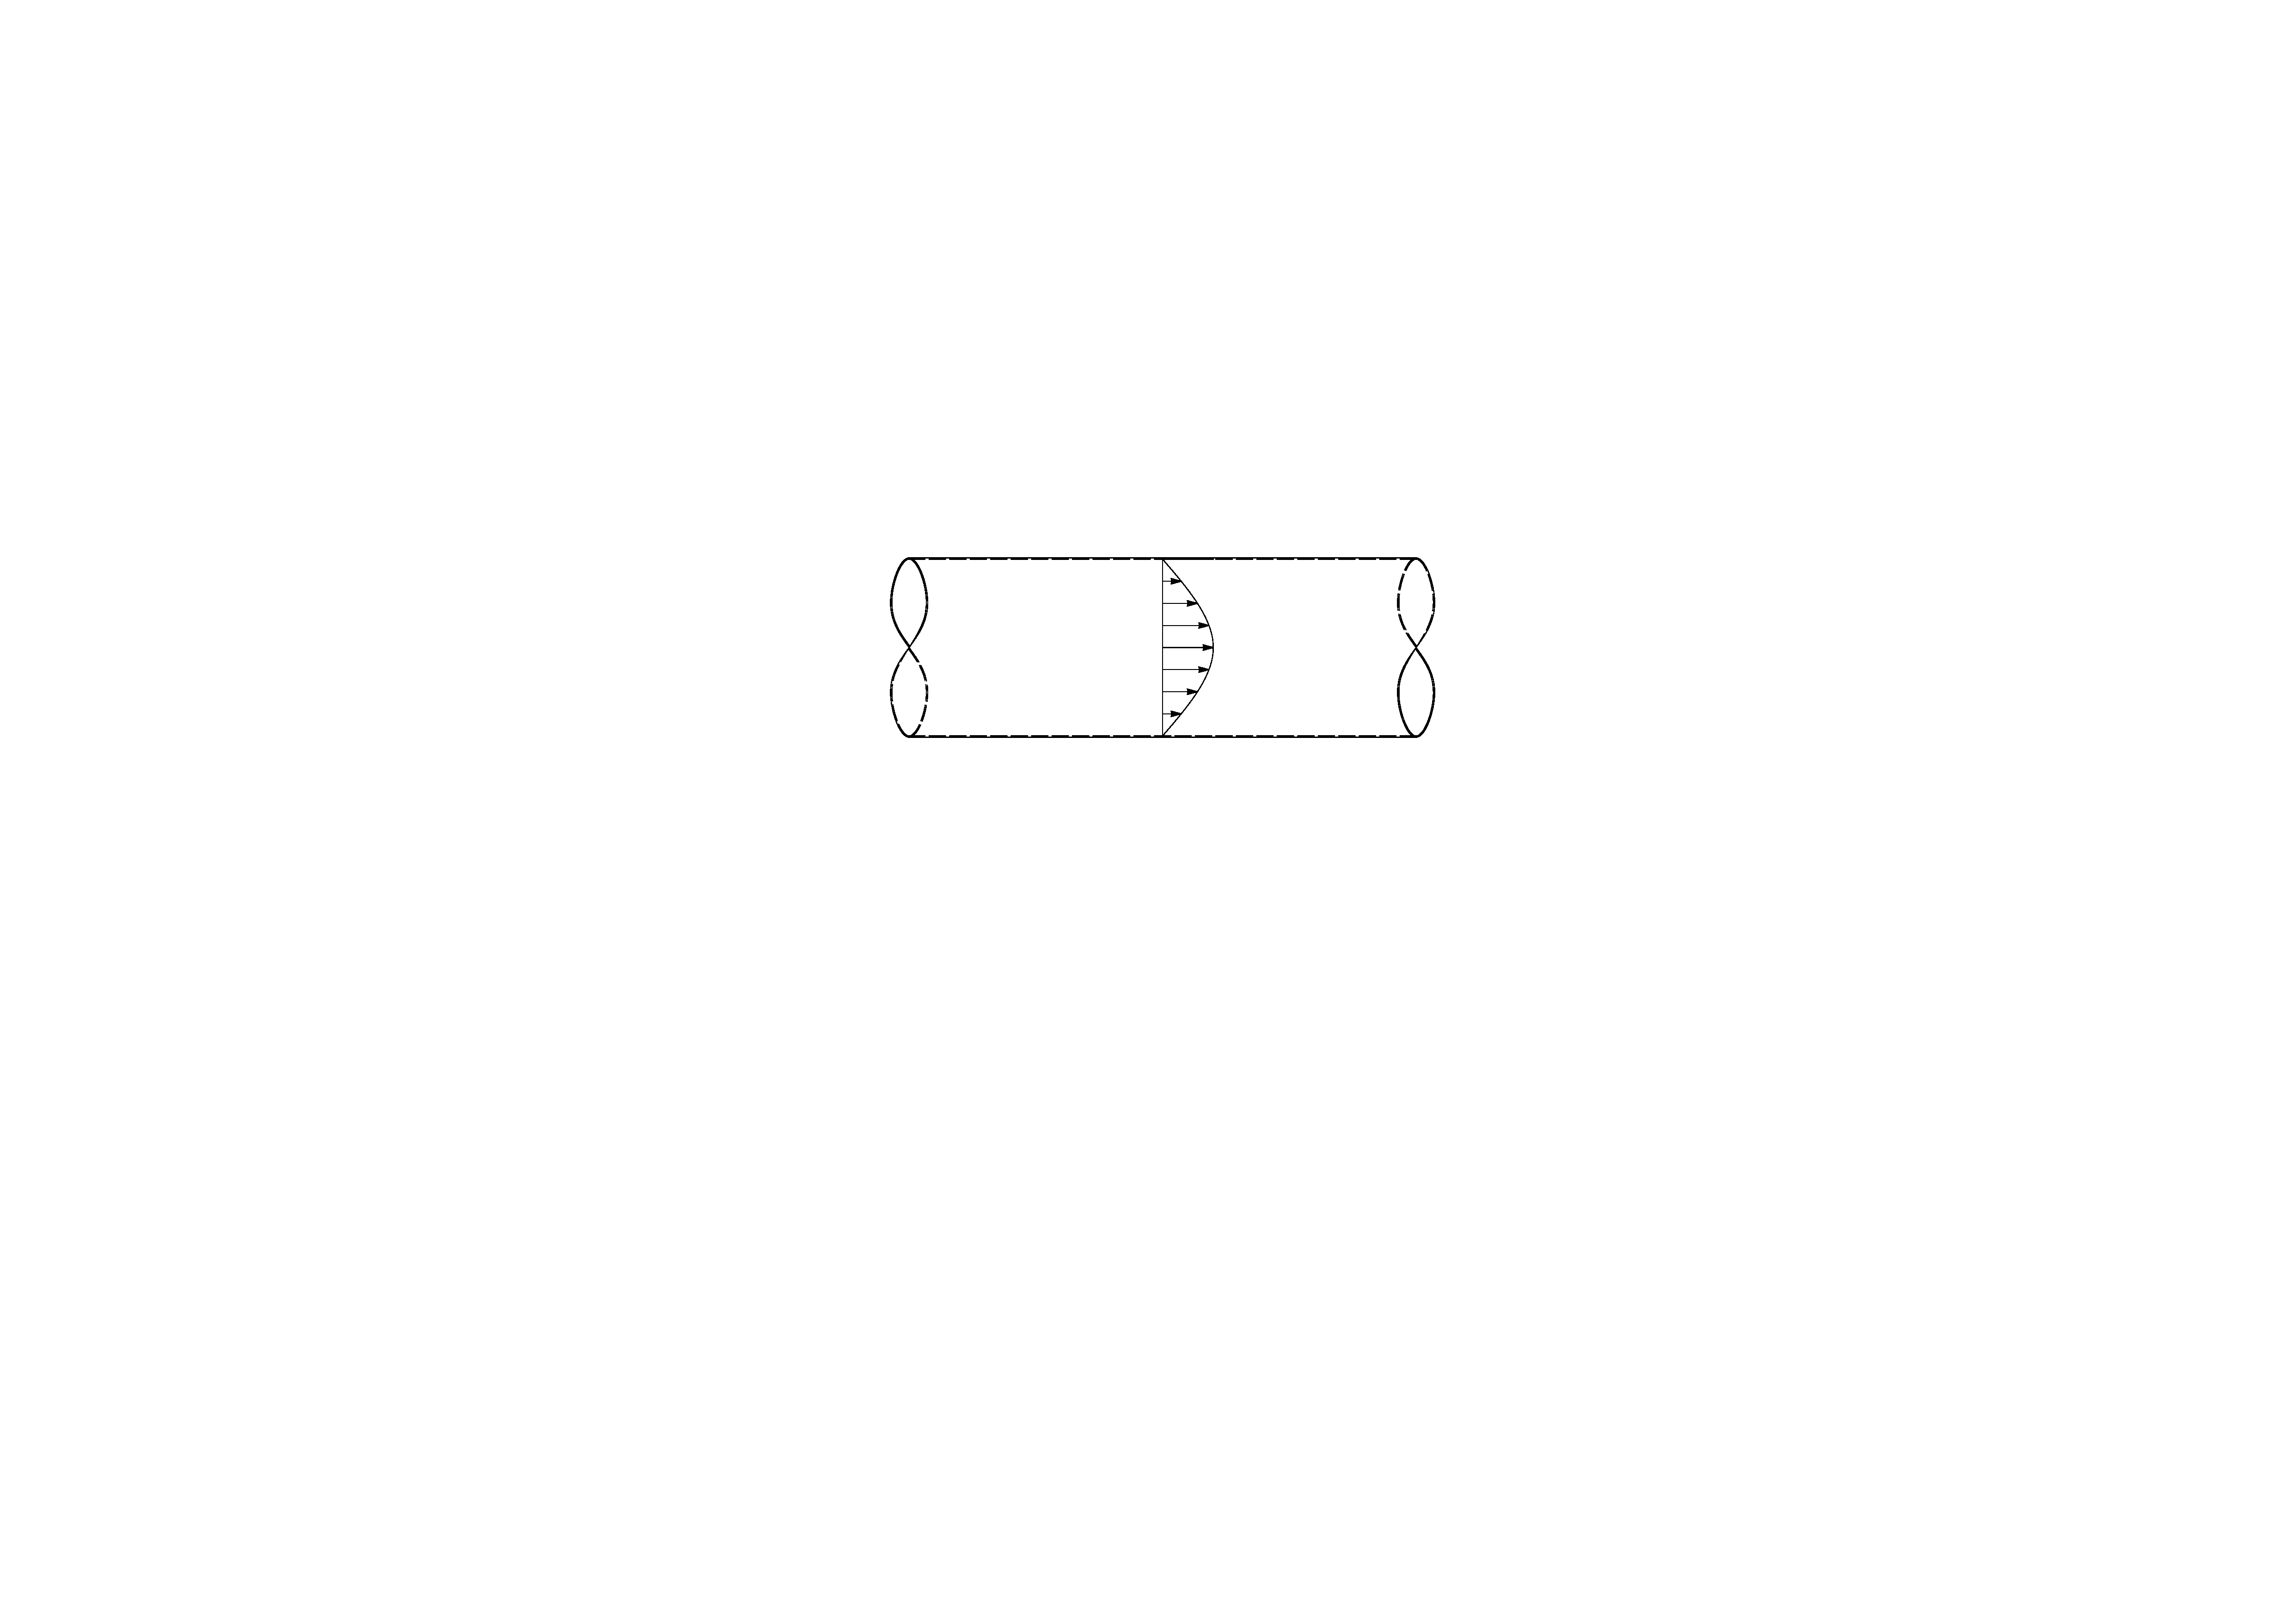
\includegraphics[width=.75\linewidth]{Figuras/EscLaminar.pdf}
        \caption{Escoamento laminar.}
        \label{fig:EscLaminar}
      \end{subfigure}
      \begin{subfigure}{.45\textwidth}
        \centering
        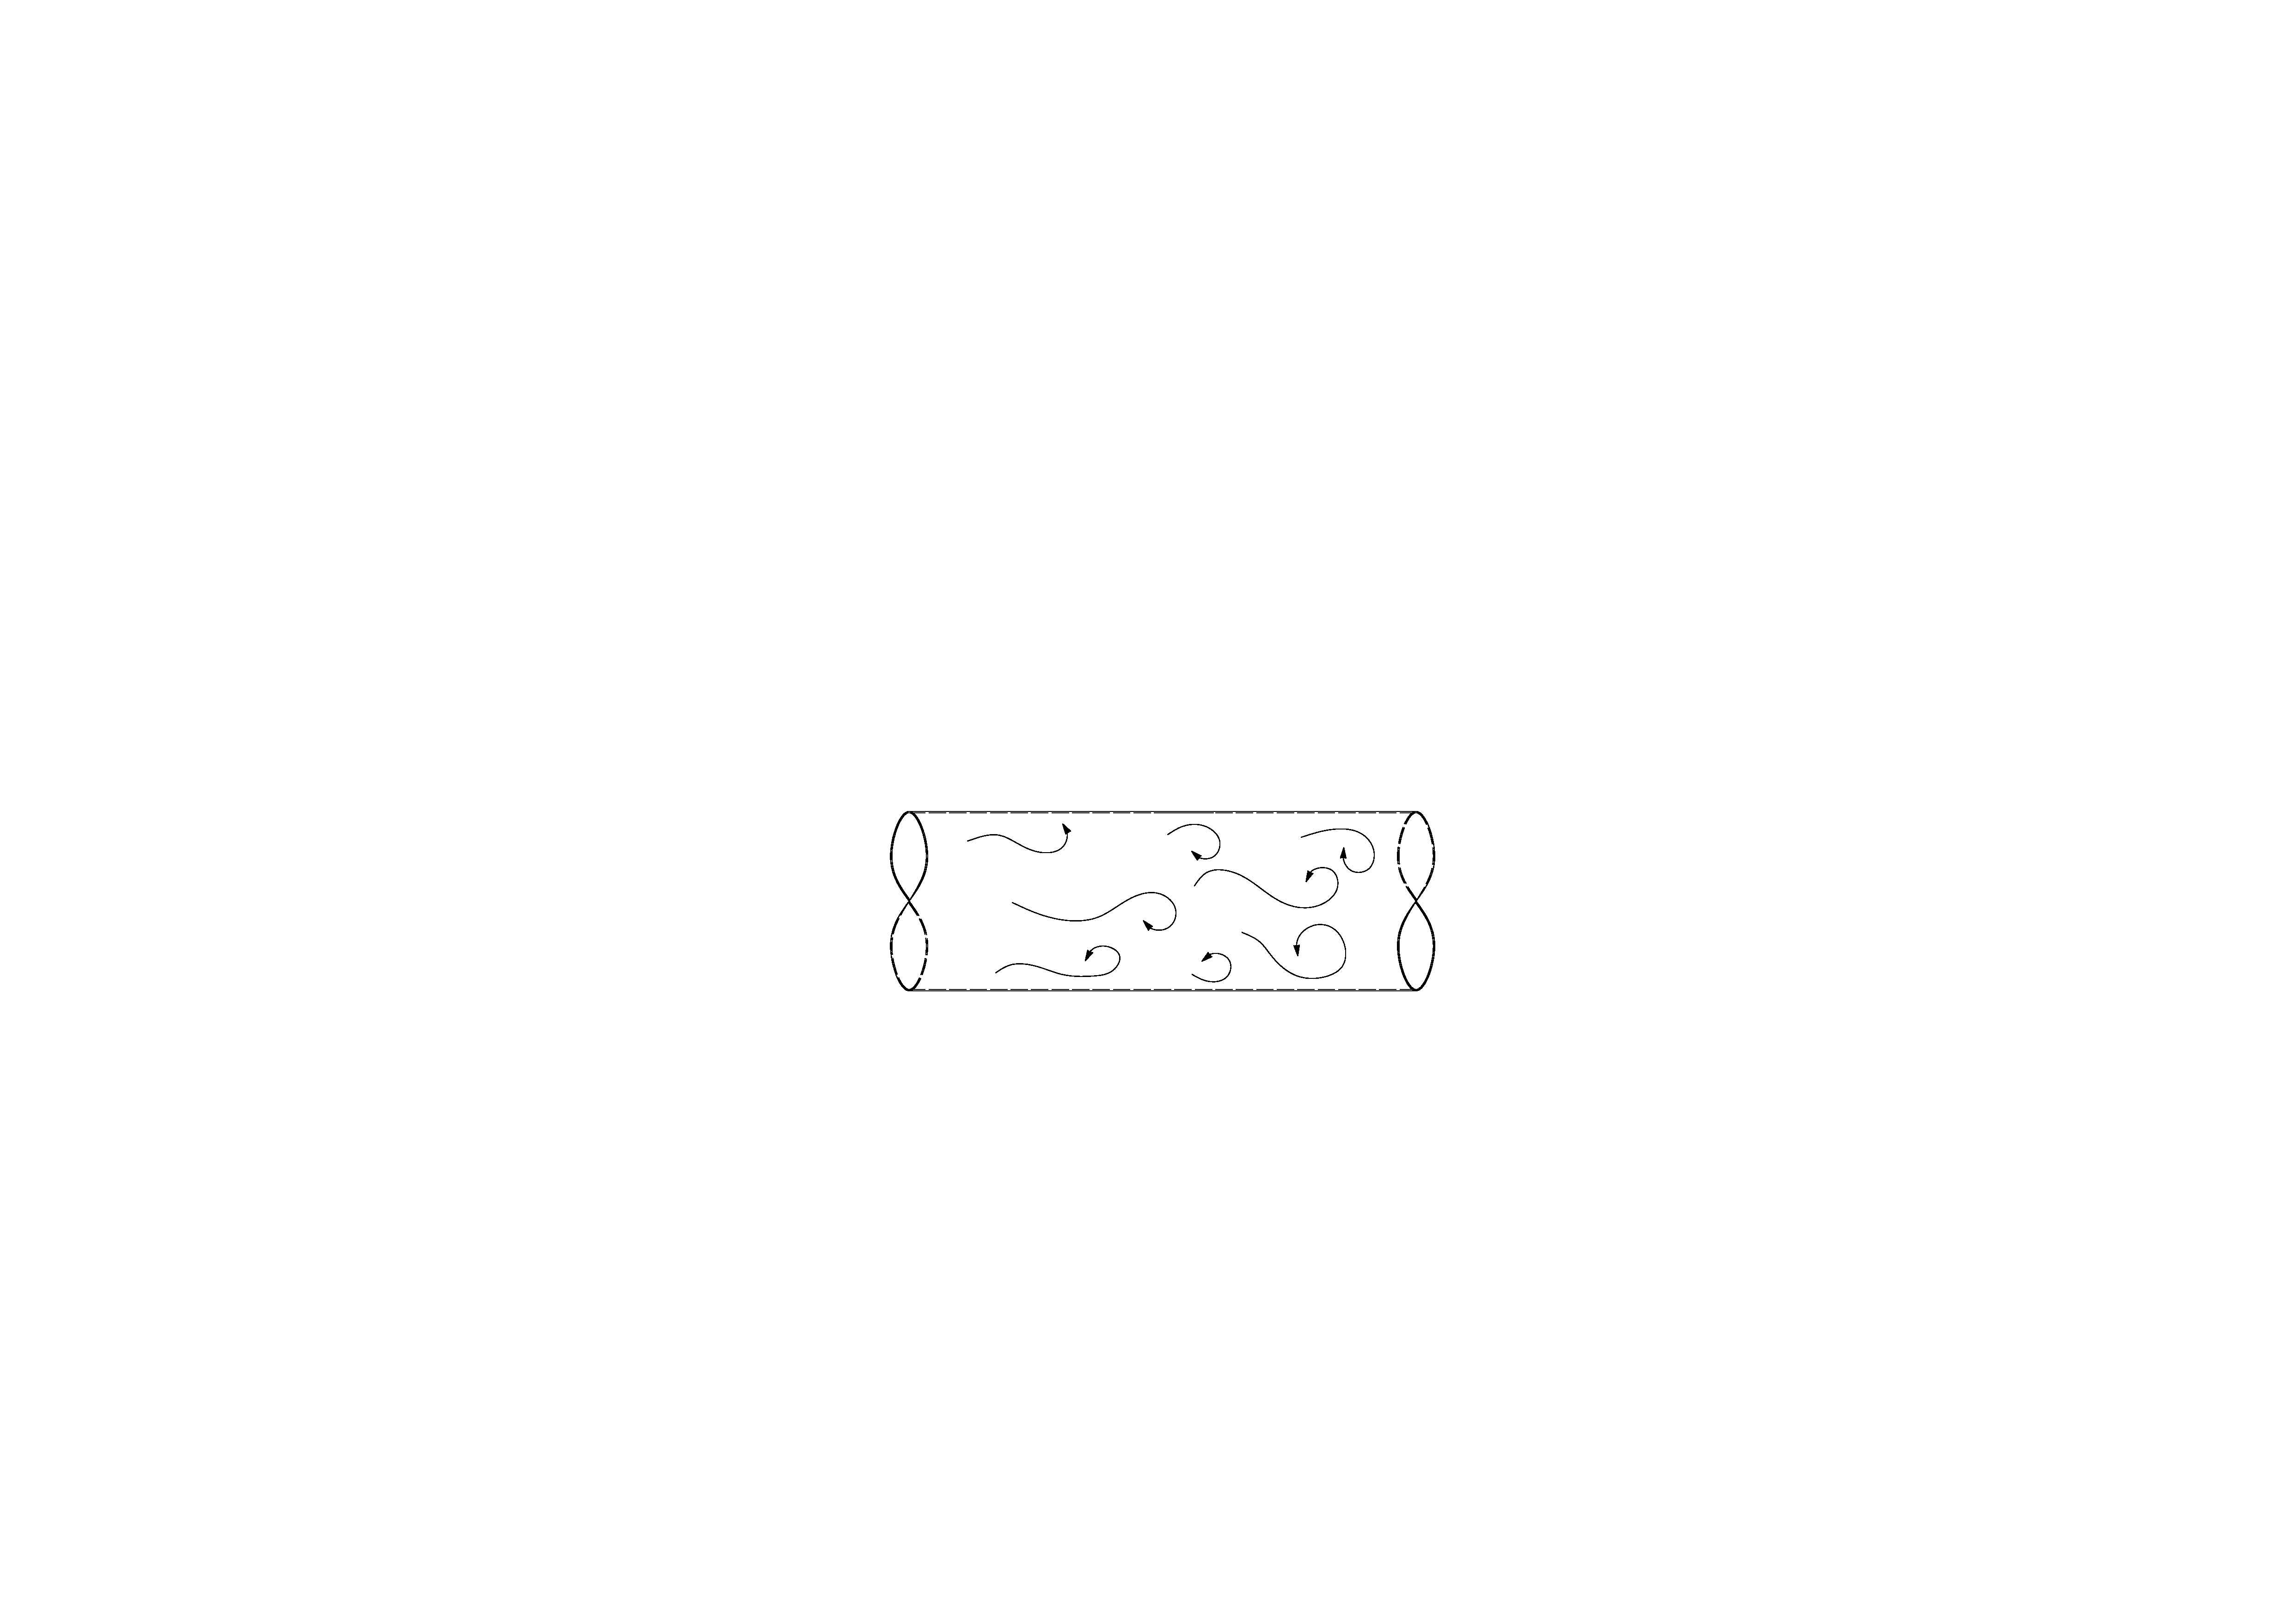
\includegraphics[width=.75\linewidth]{Figuras/EscTurbulento.pdf}
        \caption{Escoamento turbulento.}
        \label{fig:EscTurbulento}
      \end{subfigure}
    \\Fonte: Autoria Própria (\the\year).
\end{figure}

\end{document}

%==================================================================================================
\section{Objetivos}
%==================================================================================================

Esta proposta tem como objetivo principal o estudo de formulações numéricas e a implementação computacional de modo a se obter ferramentas computacionais eficientes e precisas para a simulação de problemas de interação fluido-estrutura com elevados números de Reynolds, onde possa haver efeitos de turbulência. Dentro desse escopo, alguns objetivos específicos devem ser alcançados:

\begin{itemize}
    \item Estudo das formulações estabilizadas do método dos elementos finitos para escoamentos incompressíveis com contornos móveis, com destaque para as estabilizações SUPG, LSIC, PSPG e VMS;

    \item Estudo da formulação posicional do MEF para análise dinâmica de sólidos e cascas com grandes deslocamentos;

    \item Estudo das técnicas de acoplamento particionado fluido-estrutura com malhas móveis;

    \item Estudo dos diversos modelos de turbulência no contexto do MEF;

    \item Implementação da formulação estabilizada \VMS;

    \item Implementação do modelo \LES;

    \item Acoplamento do código para mecânica dos fluidos com programa para análise não linear de estruturas de cascas;

    \item Estudo comparativo dos modelos implementados através da simulação de exemplos disponíveis na literatura.
\end{itemize}

%==================================================================================================
% METODOLOGIA
%==================================================================================================

%==================================================================================================
\chapter{Metodologia e cronograma} \label{MetodologiaCronograma}
%==================================================================================================

Tendo em vista a complexidade dos problemas em estudo, delimita-se os estudos dos problemas de interação fluido-estrutura considerando escoamento incompressível viscoso interagindo com estruturas reticuladas com grandes deslocamentos. Adota-se acoplamento particionado forte do tipo bloco-iterativo com método de malha móvel para o fluido empregando-se a descrição Lagrangiana-Euleriana Arbitrária (ALE). Essa abordagem é adotada por ser reconhecidamente robusta, modular e amplamente utilizada para análises de IFE.

Assim como os problemas a serem estudados, as implementações necessárias também são bastante complexas, sendo importante a adoção de uma metodologia de programação que aproveite os códigos disponíveis e ao mesmo tempo facilite alterações de tipos de elementos, modelos constitutivos, métodos de solução de sistemas e operações algébricas, e mais importante no contexto desta proposta, diferentes métodos de estabilização e diferentes modelos de turbulência.

Dessa forma, adota-se a linguagem de programação C++ orientada a objeto, em um sistema operacional Linux, uma vez que se é possível aproveitar diversos códigos já desenvolvidos pelo grupo de pesquisa, a saber, programa de elementos finitos para análise de escoamentos incompressíveis empregando-se elementos triangulares (2D) e tetraédricos (3D) com aproximações linear ou quadrática e programa para análise dinâmica não linear geométrica de estruturas de casca finas ou espessas empregando elementos triangulares cúbicos.

Para a solução da mecânica dos sólidos será empregado o MEF baseado em posições, aproveitando-se um programa para análise de cascas com cinemática de Reissner-Mindlin, já desenvolvido pelo grupo de pesquisa. A formulação baseada em posições emprega uma descrição Lagrangiana Total, sendo adotado o modelo constitutivo de Saint-Venant Kirchhoff  com a medida de deformação de Green-Lagrange. O elemento de casca utilizado possui 7 graus de liberdade por nó, a saber, 3 coordenadas de posição, 3 coordenadas de um vetor generalizado, inicialmente perpendicular à superfície média da casca, e 1 parâmetro de enriquecimento para permitir variação linear da deformação na direção da espessura. A aproximação das derivadas temporais do problema é feita com integrador temporal $alpha$-generalizado. O processo de solução dos sistema não linear é obtida por meio do método iterativo de Newton-Raphson. 

Já para a solução da mecânica dos fluidos fluido, parte-se de um código computacional para escoamentos bidimensionais e tridimensionais empregado a formulação estabilizada PSPG/SUPG do MEF e a descrição ALE, o que possibilita a representação de contornos móveis. Assim como no sólido, a aproximação temporal é dada pelo integrador $\alpha$-generalizado e o método de Newton-Raphson é empregado para a solução do sistema não linear. Neste código é parte desta proposta a implementação de elementos Taylor-Hood, com aproximação quadrática para velocidades e linear para pressão, a implementação da técnica de estabilização \LSIC (LSIC) para captura de vórtices, assim comoos modelos de turbulência RANS e LES e o modelo de estabilização VMS (implementações essas que já foram finalizadas).

Após o estudo e verificação isolada das ferramentas para solução do fluido e do sólido, parte-se para o acoplamento.
Para isso será adotado um modelo de acoplamento particionado forte do tipo bloco-iterativo, sendo a movimentação da malha do fluido realizada por meio de um problema fictício de elasticidade, considerando-se a malha do fluido como um sólido elástico com deslocamentos prescritos no contorno.

% \textcolor{red}{-Falar como você vai resolver o sólido (citar o programa de cascas disponível, a formulação empregada e a integração temporal adotada). Especificar se você vai implementar alguma coisa nele ou só utilizar.}

% \textcolor{red}{-Falar como você vai resolver o fluido considerando contornos móveis (citar o programa de fluido disponível, a formulação/elementos empregados e a integração temporal adotada). Especificar o que você vai implementar}

% \textcolor{red}{-Falar sobre a técnica de acoplamento a ser adotada para unir os códigos}

Será empregado o protocolo de processamento paralelo \textit{Message Passing Interface} (MPI), com utilização da biblioteca PETSc (\textit{Portable, Extensible Toolkit for Scientific Computation}) \cite{petsc-web-page}, a qual é reconhecidamente eficiente para solução de sistemas esparços que necessitem de alto desempenho computacional, tendo suporte para C++ e MPI.  As malhas serão geradas a partir do programa Gmsh \cite{geuzaine2009gmsh}, e os resultados serão interpretados graficamente por meio do visualizador Paraview \cite{ahrens2005paraview} e por meio do programa gnuPlot, no caso da geração de gráficos de linha 2D ou 3D. Nota-se que prioriza-se o uso de ferramentas computacionais livres e de código aberto para facilitar a distribuição e as atualizações da ferramenta computacional resultante.

%==================================================================================================
\section{Cronograma}
%==================================================================================================

% \textcolor{red}{As atividades estavam insuficientes para descrever o seu trabalho durante o curso (pode incluir as disciplinas, já que o cronograma é do trabalho de mestrado como todo). Adicionei outras atividades, verifique se não falta nada e atualize o cronograma (Pode incluir o exame de qualificação...).}

As atividades necessárias para se alcançar os objetivos desta pesquisa são organizadas da seguinte maneira:

\begin{enumerate}[label=\alph*.]
	\item\label{M:1} Cursar disciplinas do programa de mestrado;
	\item\label{M:2} Revisão bibliográfica a ser realizada de forma contínua ao longo de todo o trabalho, para que o mesmo se mantenha atualizado frente ao estado da arte durante toda sua execução;
	\item\label{M:3} Estudo das formulações estabilizadas do método dos elementos finitos para a solução de escoamentos incompressíveis com contornos móveis;
	\item\label{M:4} Estudo dos modelos de turbulência RANS e LES;
	\item\label{M:5} Estudo do código computacional para escoamentos incompressíveis disponível e implementações do modelo de estabilização VMS;
	\item\label{M:6} Implementação computacional dos modelos de turbulência no código de escoamentos incompressíveis;
	\item\label{M:7} Verificação dos modelos de turbulência implementados no contexto de escoamentos com contornos fixos a partir de exemplos presentes na literatura;
	\item\label{M:8} Estudo da formulação posicional do MEF para elementos de casca com cinemática de Reissner-Mindlin;
	\item\label{M:9} Exame de qualificação de mestrado;
	\item\label{M:10} Estudo e implementação do modelo de acoplamento particionado do tipo bloco-iterativo;
	\item\label{M:11} Verificação e Estudo dos modelos implementados no contexto dos problemas de iteração fluido-estrutura com elevados números de Reynolds;
	\item\label{M:12} Redação da dissertação e elaboração de artigos para revistas;
	\item \label{M:13} Defesa do mestrado.
\end{enumerate}

Essas atividades são organizadas cronologicamente, ao longo do tempo disponível para a conclusão do mestrado, de acordo com o cronograma da Tabela \ref{Cronograma}.

\definecolor{lightgray}{RGB}{153,153,153}
\definecolor{lightblue}{RGB}{126,194,216}

\begin{table}[h!]
	\caption{Cronograma de atividades}
	\fontsize{8}{14}\selectfont
	\centering
	\newcommand{\Rx}{\cellcolor{lightblue}}
	\newcommand{\Px}{\cellcolor{lightgray}}
	\begin{tabular}{|c|ccccccccc|cccccccccccc|cccc|}
		\hline
		\MR{2}{*}{Item} & \MC{9}{c|}{2022} & \MC{12}{c|}{2023} & \MC{4}{c|}{2024}                                                                                                                                     \\ \cline{2-26}
		                & A                & M                 & J                & J   & A   & S   & O   & N   & D   & J   & F   & M   & A   & M   & J   & J   & A   & S   & O   & N   & D   & J   & F   & M   & A   \\ \hline
		\ref{M:1}       & \Rx              & \Rx               & \Rx              & \Rx & \Rx & \Rx & \Rx & \Rx & \Rx &     &     &     &     &     &     &     &     &     &     &     &     &     &     &     &     \\ \hline
		\ref{M:2}       & \Rx              & \Rx               & \Rx              & \Rx & \Rx & \Rx & \Rx & \Rx & \Rx & \Rx & \Rx & \Rx & \Rx & \Rx & \Rx & \Rx & \Px & \Px & \Px & \Px & \Px & \Px & \Px & \Px &     \\ \hline
		\ref{M:3}       &                  &                   &                  &     & \Rx & \Rx & \Rx & \Rx & \Rx & \Rx & \Rx &     &     &     &     &     &     &     &     &     &     &     &     &     &     \\ \hline
		\ref{M:4}       &                  &                   &                  &     &     &     &     & \Rx & \Rx & \Rx & \Rx & \Rx & \Rx & \Rx &     &     &     &     &     &     &     &     &     &     &     \\ \hline
		\ref{M:5}       &                  &                   &                  &     &     &     &     &     &     &     & \Rx & \Rx & \Rx & \Rx &     &     &     &     &     &     &     &     &     &     &     \\ \hline
		\ref{M:6}       &                  &                   &                  &     &     &     &     &     &     &     &     &     &     & \Rx & \Rx & \Rx & \Px & \Px & \Px &     &     &     &     &     &     \\ \hline
		\ref{M:7}       &                  &                   &                  &     &     &     &     &     &     &     &     &     &     &     & \Rx & \Rx &     &     &     &     &     &     &     &     &     \\ \hline
		\ref{M:8}       &                  &                   &                  &     &     &     &     &     &     &     &     &     &     & \Rx & \Rx & \Rx &     &     &     &     &     &     &     &     &     \\ \hline
		\ref{M:9}       &                  &                   &                  &     &     &     &     &     &     &     &     &     &     &     &     &     & \Px &     &     &     &     &     &     &     &     \\ \hline
		\ref{M:10}      &                  &                   &                  &     &     &     &     &     &     &     &     &     &     &     &     &     & \Px & \Px & \Px & \Px &     &     &     &     &     \\ \hline
		\ref{M:11}      &                  &                   &                  &     &     &     &     &     &     &     &     &     &     &     &     &     &     &     &     & \Px & \Px & \Px & \Px &     &     \\ \hline
		\ref{M:12}      & \Rx              & \Rx               & \Rx              & \Rx & \Rx & \Rx & \Rx & \Rx & \Rx & \Rx & \Rx & \Rx & \Rx & \Rx & \Rx & \Rx & \Px & \Px & \Px & \Px & \Px & \Px & \Px & \Px &     \\ \hline
		\ref{M:13}      &                  &                   &                  &     &     &     &     &     &     &     &     &     &     &     &     &     &     &     &     &     &     &     &     &     & \Px \\ \hline
	\end{tabular}
	\label{Cronograma}
\end{table}

\begin{minipage}{\textwidth}
	\fontsize{8}{14}\selectfont
	\centering
	\colorbox{lightblue}{\rule{0pt}{10pt}\rule{10pt}{0pt}} Já realizado \quad
	\colorbox{lightgray}{\rule{0pt}{10pt}\rule{10pt}{0pt}} Pendente \quad
\end{minipage}

%==================================================================================================
\section{Justificativa}
%==================================================================================================

Os avanços na área da engenharia colocam em evidência a necessidade cada vez maior de se determinar de forma precisa as variáveis necessárias ao dimensionamento de estruturas, sejam referentes à resistência dos materiais utilizados, ou às solicitações atuantes. Nesse sentido, em diversas ocasiões, os efeitos advindos da interação fluido-estrutura (IFE) são responsáveis por submeter estruturas a esforços consideráveis, o que demanda que esses efeitos sejam adequadamente estudados. Dessa forma, a análise desse tipo de problema via métodos computacionais se mostra promissor, uma vez que estudos experimentais normalmente são dispendiosos e pouco flexíveis quanto às suas aplicações.

Dentre os métodos empregados, pode-se destacar o dos Elementos Finitos (MEF), com aplicações tanto para modelar o sólido como para o fluido. Esse método ganha atenção, uma vez que pode se adequar com certa facilidade à problemas de geometria complexa, garantindo ainda facilidade para aplicação de condições de contorno.

Embora no contexto da mecânica dos fluidos, a utilização do MEF segundo o método de Bubnov-Galerkin possa gerar oscilações espúrias, decorrentes dos termos convectivos, de ondas de choque nos casos compressíveis, ou da interpolação da pressão por espaços de funções inadequados nos casos incompressíveis, todos esses problemas já dispõem de técnicas consistentes para que sejam evitados. Como exemplos, destacam-se a técnica SUPG para estabilização da convecção, a técnica PSPG ou o uso de elementos Taylor-Hood para estabilização da pressão nos escoamentos incompressíveis e a introdução de operadores de captura de choque para os casos compressíveis.

Entretanto, mesmo que diversos trabalhos tenham sido realizados, resultando em grandes avanços na área, alguns desafios se mantêm, como o elevado custo computacional relacionado à simulações de IFE, o que demanda muito tempo pra a obtenção de resultados, inviabilizando sua aplicação na etapa de elaboração de muitos projetos usuais de engenharia. Nesse cenário, problemas de escoamento turbulentos se tornam ainda mais custosos, devido à alguns fenômenos como a manifestação de vórtices, geralmente tridimensionais, de forma desordenada, instável e em uma grande amplitude de escalas. Assim necessita-se de malhas muito refinadas para capturar a ocorrência dessas estruturas. Para que a simulação desses problemas seja estável em qualquer nível de discretização, e possa resultar em respostas consistentes a custos computacionais aceitáveis, faz-se necessária a adoção de modelos de turbulência, como  aqueles baseados na decomposição de Reynolds (RANS) ou em grandes vórtices (LES), ou de técnicas multiescala adequadas.

Já no contexto da mecânica dos sólidos, diversas técnicas são possíveis para abordar o problema, \eg\ o MEF corrotacional. No entanto considerar rotações nodais finitas e uma matriz de massa variável podem dificultar a aplicação dessa abordagem. Sendo assim, a utilização do MEF baseado em posições se torna interessante, uma vez que considera intrinsecamente a não linearidade geométrica, além de possuir uma matriz de massa constante, facilitando o processo de integração temporal.

Para o acoplamento entre fluido e estrutura, o processo de acoplamento particionado se torna viável na presente proposta, uma vez que se pode utilizar diferentes códigos que funcionam independentemente entre si, tanto para solução de problemas de fluidos, quanto para problemas de sólidos, e que podem ser acoplados de maneira eficiente. Isso se justifica pela presença de códigos já desenvolvidos pelo grupo de pesquisa do Departamento de Engenharia de Estruturas (SET), capazes de resolver isoladamente problemas da mecânica dos sólidos e dos fluidos. Também se opta pelo processo de acoplamento particionado forte, uma vez que se mostra eficaz na resolução de problemas fortemente acoplados.

Além disso, a utilização de malhas móveis para o fluido, por meio da descrição ALE, se mostra como uma alternativa viável, uma vez que permite que a malha do fluido se movimente dinamicamente para acomodar a movimentação da interface fluido-sólido. Sendo a movimentação dada pelo esquema de movimentação suave de Laplace, com uma modificação que confere maior rigidez aos elementos menores da malha, o que previne distorções excessivas de elementos pequenos, mantendo, consequentemente, a qualidade da malha.

Sendo assim, o presente trabalho é justificado ao propor o desenvolvimento de uma ferramenta computacional eficiente e precisa, aplicada a problemas de IFE com escoamentos turbulentos com a opção de se aplicar modelo de turbulência para redução do custo computacional. Igualmente, fica justificado a proposta de estudar e comparar os diferentes modelos e estabilizações a serem implementadas quando da aplicação a problemas de IFE. A presente pesquisa visa ainda aprimorar as ferramentas computacionais que estão sendo desenvolvidas pelo grupo de pesquisa do SET da Escola de Engenharia de São Carlos (EESC) da Universidade de São Paulo (USP), ampliando seu leque de aplicações.

% Outro desafio que se pode destacar é referente aos problemas de acoplamento, uma vez que os modelos constitutivos que regem tanto os sólidos quanto os fluidos são distintos, assim como as variáveis empregadas para descrever o comportamento de cada um. Também verifica-se que o sistema de equações fundamental para o estudo desses problemas, ou não possui solução analítica, ou essa só pode ser obtida para casos simples e com hipóteses bastante simplificadoras, sem muita possibilidade de generalizações.